%! alt The complex plane, with the circle of radius 20 centred at 3 - 8i. Four segments of length 10 and the same direction start on the real axis at k. For k = -16 the segment touches the circle at its midpoint. For k = 0 it lies inside the circle, so there is no solution. For k = 9 its far end lies on the circle. For k = 15 it crosses the circle once.
%! after_paragraph 2
%! scale 1/6
% The shared preamble of every Kyuclid figure. pipeline/figures turns these colours into theme-aware paint,
% and refuses any other colour, so draw only with them:
%   figink (lines and labels), figaux (construction lines), figaccent (the object the argument turns on),
%   figtint and figaccenttint (light fills).
\documentclass[border=1.5pt]{standalone}
\usepackage{tkz-euclide}
\definecolor{figink}{RGB}{0,0,0}
\definecolor{figaux}{RGB}{85,85,85}
\definecolor{figaccent}{RGB}{192,57,43}
\definecolor{figtint}{RGB}{221,221,221}
\definecolor{figaccenttint}{RGB}{245,213,208}
% tkz-euclide's defaults draw circles, compasses and marks in 50% grey and fill points with a tint.
\makeatletter
\def\tkz@otherlinecolor{figink}
\def\tkz@euc@circlecolor{figink}
\def\tkz@euc@compasscolor{figink}
\def\tkz@euc@mkcolor{figink}
\def\tkz@mk@fill{figink}
\def\tkz@euc@pointfillcolor{figink}
\makeatother
\tkzSetUpLine[color=figink,line width=.7pt]
\tkzSetUpArc[color=figink,line width=.7pt]
\tkzSetUpCompass[color=figink,line width=.5pt]
\tkzSetUpPoint[color=figink,fill=figink,size=3.1pt]
\tikzset{
  every picture/.style={line cap=round,line join=round,color=figink},
  circle style/.append style={color=figink,line width=.7pt},
  aux/.style={color=figaux,line width=.45pt,dash pattern=on 2.6pt off 2pt},
  key/.style={color=figaccent,line width=1pt},
  mk/.style={color=figink,line width=.5pt},
  lbl/.style={color=figink,inner sep=2.2pt},
  len/.style={color=figink,inner sep=1.5pt,font=\small},
}

\begin{document}
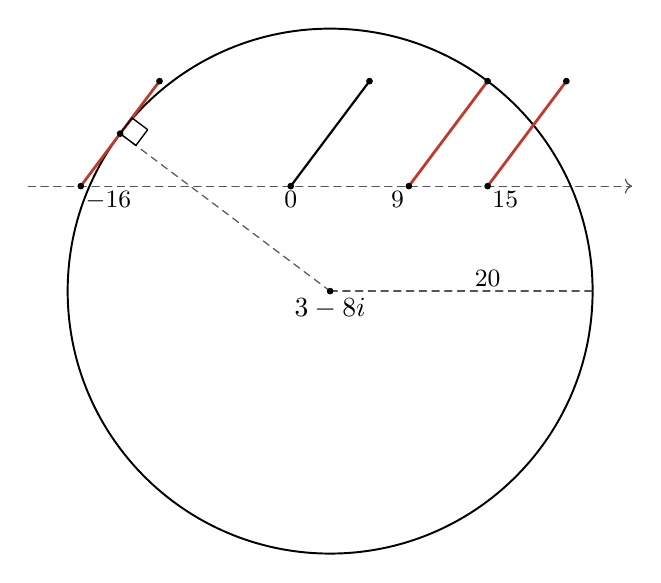
\begin{tikzpicture}
\tkzDefPoint(0.50000000,-1.3333333){C} %! C = (3, -8)
\tkzDefPoint(3.8333333,-1.3333333){R} %! R = (23, -8)
\tkzDefPoint(-3.3333333,0.0){XL} %! XL = (-20, 0)
\tkzDefPoint(4.3333333,0.0){XR} %! XR = (26, 0)
\tkzDefPoint(-2.6666667,0.0){A1} %! A1 = (-16, 0)
\tkzDefPoint(-1.6666667,1.3333333){B1} %! B1 = (-10, 8)
\tkzDefPoint(-2.1666667,0.66666667){T} %! T = mid(A1, B1)
\tkzDefPoint(0.0,0.0){A2} %! A2 = (0, 0)
\tkzDefPoint(1.0000000,1.3333333){B2} %! B2 = (6, 8)
\tkzDefPoint(1.5000000,0.0){A3} %! A3 = (9, 0)
\tkzDefPoint(2.5000000,1.3333333){B3} %! B3 = (15, 8)
\tkzDefPoint(2.5000000,0.0){A4} %! A4 = (15, 0)
\tkzDefPoint(3.5000000,1.3333333){B4} %! B4 = (21, 8)
%! fact on_circle(R, C, 20)
%! fact tangent(C, 20, A1, B1)
%! fact on_circle(T, C, 20)
%! fact on_segment(T, A1, B1)
%! fact dist(C, B2) < 20
%! fact dist(C, A2) < 20
%! fact on_circle(B3, C, 20)
%! fact dist(C, A3) < 20
%! fact dist(C, A4) < 20
%! fact dist(C, B4) > 20
%! fact dist(A1, B1) == 10
%! fact dist(A2, B2) == 10
%! fact dist(A3, B3) == 10
%! fact dist(A4, B4) == 10
\draw[aux,->] (XL) -- (XR);
\tkzDrawCircle(C,R)
\tkzDrawSegment[aux](C,T)
\tkzDrawSegment[aux](C,R)
\tkzDrawSegment[line width=.8pt](A2,B2)
\tkzDrawSegments[key](A1,B1 A3,B3 A4,B4)
\tkzMarkRightAngle[size=.25,mk](C,T,B1)
\tkzDrawPoints(C,T,A1,B1,A2,B2,A3,B3,A4,B4)
\tkzLabelPoint[below,lbl](C){$3-8i$}
\tkzLabelPoint[below right,len](A1){$-16$}
\tkzLabelPoint[below,len](A2){$0$}
\tkzLabelPoint[below left,len](A3){$9$}
\tkzLabelPoint[below right,len](A4){$15$}
\tkzLabelSegment[above,pos=.6,len](C,R){$20$}
\end{tikzpicture}
\end{document}
